% compile with: pdflatex -shell-escape filename.tex
\documentclass[crop,tikz,convert=pdf2svg]{standalone}
\usetikzlibrary{automata}

\tikzset{
  ->,
  >=latex,
  every state/.style={thick, fill=gray!10},
  initial text=$ $,
  node distance=3cm,
}

\begin{document}

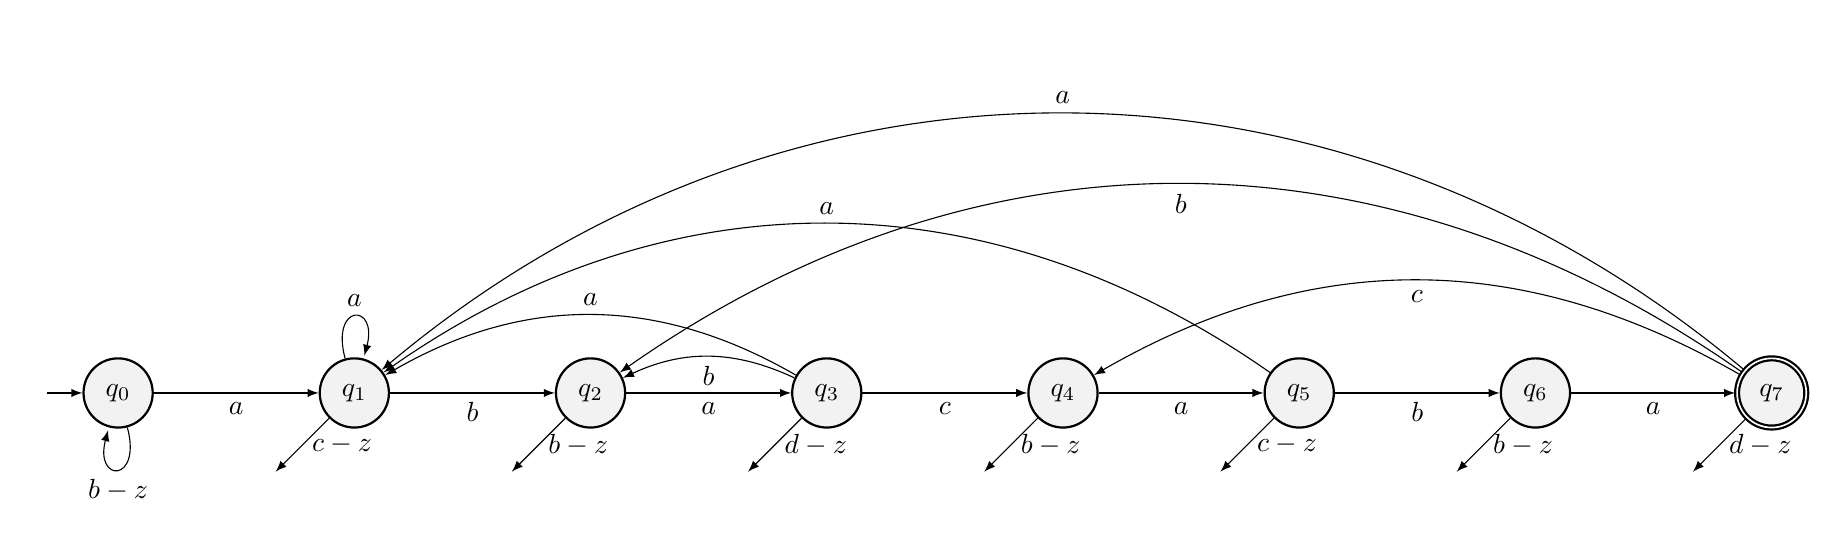
\begin{tikzpicture}
  \node[state, initial] (q0) {$q_0$};
  \node[state, right of=q0] (q1) {$q_1$};
  \node[state, right of=q1] (q2) {$q_2$};
  \node[state, right of=q2] (q3) {$q_3$};
  \node[state, right of=q3] (q4) {$q_4$};
  \node[state, right of=q4] (q5) {$q_5$};
  \node[state, right of=q5] (q6) {$q_6$};
  \node[state, accepting, right of=q6] (q7) {$q_7$};
  \draw
  (q0) edge[below] node{$a$} (q1)
  (q0) edge[loop below] node{$b-z$} (q0)

  (q1) edge[below] node{$b$} (q2)
  (q1) edge[loop above] node{$a$} (q1)

  (q2) edge[below] node{$a$} (q3)

  (q3) edge[below] node{$c$} (q4)
  (q3) edge[bend right, above] node{$a$} (q1)
  (q3) edge[bend right=25, below] node{$b$} (q2)

  (q4) edge[below] node{$a$} (q5)

  (q5) edge[below] node{$b$} (q6)
  (q5) edge[bend right=35, above] node{$a$} (q1)

  (q6) edge[below] node{$a$} (q7)

  (q7) edge[bend right=40, above] node{$a$} (q1)
  (q7) edge[bend right=35, below] node{$b$} (q2)
  (q7) edge[bend right, below] node{$c$} (q4)
  ;

  %% arrows pointing nowhere
  \draw (q1) edge[right] node{$c-z$} ++ (-1, -1);
  \draw (q2) edge[right] node{$b-z$} ++ (-1, -1);
  \draw (q3) edge[right] node{$d-z$} ++ (-1, -1);
  \draw (q4) edge[right] node{$b-z$} ++ (-1, -1);
  \draw (q5) edge[right] node{$c-z$} ++ (-1, -1);
  \draw (q6) edge[right] node{$b-z$} ++ (-1, -1);
  \draw (q7) edge[right] node{$d-z$} ++ (-1, -1);
\end{tikzpicture}

\end{document}
